\chapter{Missionsdesign und Simulation}

%\section{Bewertungsstrategie}
	%Die Strategie besteht draus mehrere Simulationen per GMAT für untershciedliche Koonfigs durchzuführen. Die Bewertung fokusiertsich auf die Machbarkeit des De-orbiting (seihe TODOS.txt)\\
	%	\subsection{Kriterien der Bewertung}
%-------------------------------------------------------------Missionsbeschreibung

\section{Missionsbeschreibung}

Ziel der Mission ist es defekte, nicht kooperative Satelliten von Megakonstellationen (z.B.: Starlink) abzubremsen, sodass sie in der Erdatmosphäre verglühen und das Kollisionsrisiko minimiert wird. Das Höhen- und Gewichtsintervall wurden auf 400-1400 $km$, bzw. 50-5000 $kg$ festgelegt, da alle Satelliten bisher geplanter Megakonstellationen innerhalb dieser Intervalle befinden.
Es wird angenommen, dass sich der CubeSat und das Ziel zu Beginn in derselben Umlaufbahn befinden und nur wenige Kilometer voneinander entfernt sind. Das Haupttriebwerk wird für RDV und Docking nicht verwendet, sodass für den Deorbit Vorgang die gesamte Kraftstoffmenge zur Verfügung steht. Sobald beide Satelliten miteinander Verbunden sind richten sie sich so aus, dass das Haupttriebwerk des CubeSats entgegen der Bewegungsrichtung wirkt. Als nächstes beginnt der eigentliche Deorbit Vorgang. Hier fängt auch die jeweilige Simulation an. Da die Solarzellen den Antrieb nicht dauerhaft versorgen können, wird ein Brennintervall von 58° um den höchsten Punkt festgelegt. Jeder Brennvorgang verringert die Geschwindigkeit und senkt somit das Perigäum ab. Die Mission ist erfolgreich, wenn das Perigäum eine Höhe von 180 $km$ erreicht hat. Die Simulation wird nach zehn Jahren abgebrochen, wenn die Mission bis dahin nicht erfolgreich war. 
Zuerst wird eine Mission simuliert, die eine kreisförmige Umlaufbahn annimmt und das Höhenintervall in 50 $km$ Schritten erhöht. Die Masse wird von 50 bis 550 $kg$ in 25 $kg$ und von 600 bis 5000 $kg$ in 100 $kg$ Schritten erhöht.
Mit der zweiten Mission wird betrachtet, wie sich die Deorbitzeit für ausgewählte Massen verhält, wenn die Exzentrizität verändert wird. Das Höhenintervall beschreibt hierbei die Höhe des Perigäums und die Exzentrizität wird von 0.025 bis 0.3 betrachtet.
	
			
%-------------------------------------------------------------GMAT
\section{GMAT}
		\subsection{Beschreibung der Software}
		Der GMAT Mission Planner ist ein Open Source Programm, welches von der NASA entwickelt wird \cite{Hughes.}. Das Programm ist dazu da um Trajektorien von Satelliten zu berechnen und optimieren. Der Missionsraum umfasst das gesamte Sonnensystem und erlaubt es die Gravitationseinflüsse von allen größeren Himmelskörpern in die Berechnungen mit einfließen zu lassen. 
Die Eingabe der gewünschten Parameter erfolgt über ein GUI oder ein benutzerdefiniertes Skript. Die Skriptsprache von GMAT lehnt an der von MathWorks MATLAB(R) an.
Das GUI beinhalted einen 3D Plot und einen 2D Plot. Der 3D Plot zeigt die Position und Trajektorie des Satellitens im dreidimensionalen Raum während der 2D Plot eine Projektion der Trajektorie auf die Oberfläche eines gewählten Himmelskörpers zeigt.

\begin{figure}[!h]
	\centering
		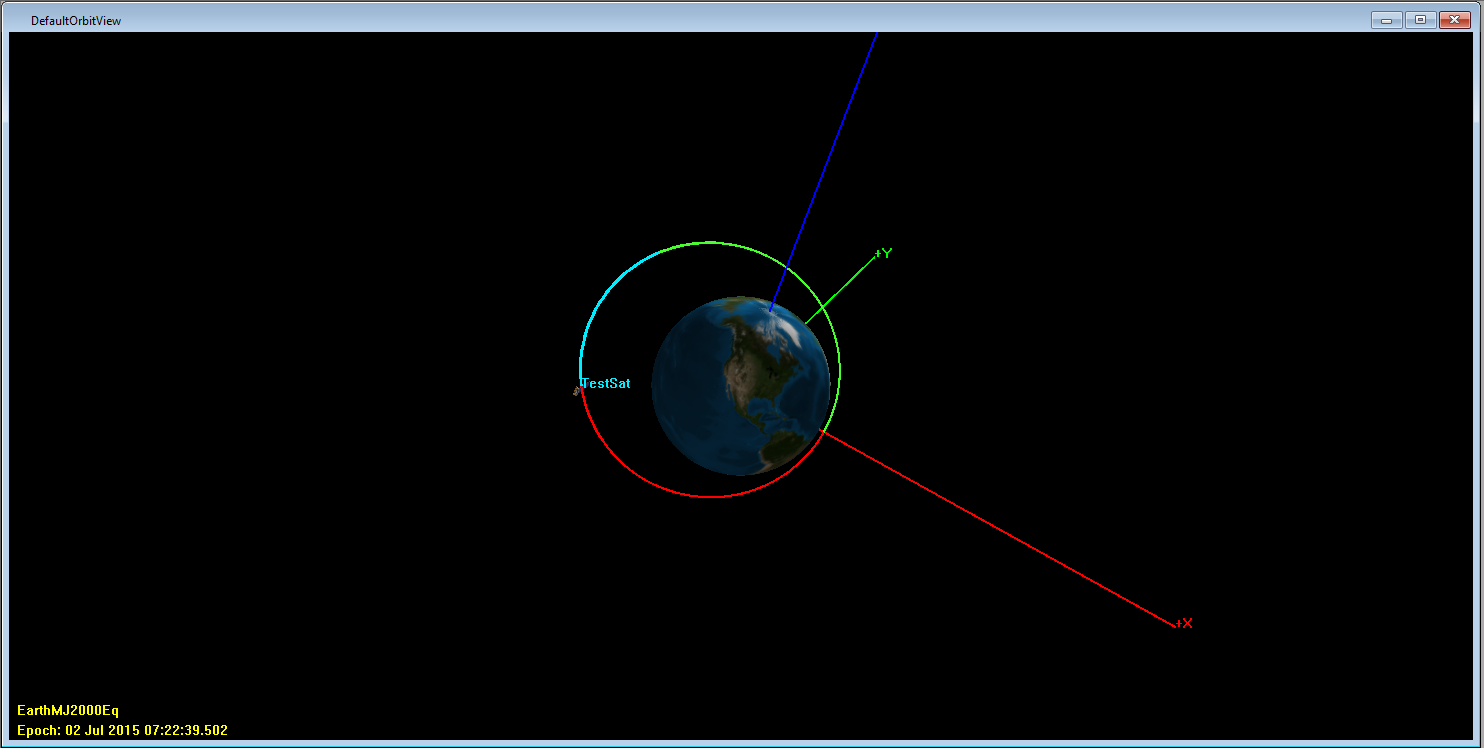
\includegraphics[width=1.00\textwidth]{graphics/GMAT/GMAT_OrbitView2.PNG}
		\caption{3D Plot eines Satelliten in einer exzentrischen Umlaufbahn um die Erde}
			\label{fig:OrbitView2}
\end{figure}


Im GUI finden sich drei Reiter: ’Resources’, ’Mission’ und ’Output’.\\
In dem Resources Reiter werden alle Ressourcen die für die Mission benötigt werden eingestellt. Dazu gehören die Schubdüsen, Tanks, Startumlaufbahn des Satelliten und andere Dinge, die während der Mission im Hintergrund wichtig sind.\\
Im Missions Reiter werden nacheinander die auszuführenden Befehle aufgelistet. Diese können auch mit Logikoperatoren wie While oder For Schleifen wiederholt werden.\\
Im Output Tab finden sich nach dem Missionsdurchlauf die Ausgaben die im Laufe der Mission erfasst worden sind wieder. 


%-------------------------------------------------------------Kreisorbitskript

\subsection{Missionsskript 1}

In dem erstem Missionsskript geht es darum, ausgehend von einer kreisförmigen Erdumlaufbahn, zu testen wie lange es dauert mit der in (verweis) gewählten Konfiguration Trümmerteile von 50 bis 5000kg zu deorbiten. Die gewählten Starthöhen liefen von 400 bis 1400km.\\

\begin{figure}[!h]
	\centering
		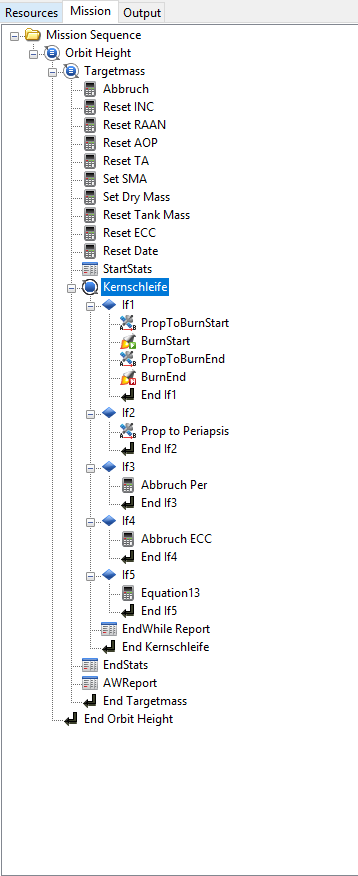
\includegraphics[width=0.35\textwidth]{graphics/GMAT/GMAT_Skript_Kreis.PNG}
		\caption{Deorbitskript - kreisförmiger Startorbit}
			\label{fig:GMAT_Skript_Kreis}
\end{figure}


Bevor die Mission in die Schleifen geht wird die Starthöhe über $Initial Orbitheight$ festgelegt. Danach geht es in die $Orbit Height$-Schleife und die Startmasse wird festgelegt.
Die nächste Schleife durchläuft alle Massen. Die Endwerte für beide Schleifen werden in $End\_mass$ und $End\_height$ festgelegt. Das Inkrement erfolgt am Ende jeder Schleife in $Inkrement mass$ bzw $Inkrement height$.\\
Im Kern diesen Skriptes steht die Whileschleife:\\
Nach einer Überprüfung des Treibstoffstands wird der Satellit mit dem ersten Propagator Befehl bis auf eine wahre Anomalie von 151 Grad vorangebracht. 
Danach wird der Schubbefehl gestartet und der Propagator $ProptoBurnEnd$ lässt den Satelliten, während dieser Schub gibt, bis zu einer wahren Anomalie von 209° vorlaufen. Sollte der Treibstoff zuvor auf 0 fallen wird dieser Vorgang abgebrochen.
Danach wird der Schub beendet.\\
Aufgrund einiger Fehler, die während des Testens dieses Skripts aufgetreten sind, folgen jetzt einige If Abfragen, die als Abbruchbedingungen der Kernschleife dienen.
Die erste überprüft ob das Perigäum des Satelliten größer als 6558 ist. Ist dies der Fall wird der Fortlauf bis zum Perigäum durchgeführt. Die Zweite If Abfrage überprüft das Gegenteil, also ob das Perigäum kleiner oder gleich 6558 ist. Ist dies der Fall wird die Variable “Abbruch” auf 1 gesetzt. Der Grund für diese beiden If Abfragen liegt darin, dass die While Schleife bei einigen Simulationen nicht auf einen zu niedrige Wert reagiert hat. Außerdem kam es vor, dass die Simulation immer langsamer wurde, wenn der Satellit bei einer kleinen Großen Halbachse zum Perigäum navigiert ist. Das wurde dadurch umgangen, dass nur zum Perigäum navigiert wird, wenn diese über 6558 ist. \\
Die nächste If Abfrage überprüft ob die Exzentrizität niedriger als 0.0025 ist. Ist dies der Fall wird der Wert “Abbruch” auf 2 gesetzt. Mit dieser If-Abfrage wird ein Fehler umgangen, der bei den niedrigen Zielhöhen häufiger aufgetreten ist. Ab einem gewissen Punkt in der Simulation von geringen Höhen verringert sich die Exzentrizität wieder, da durch atmosphärischen Drag das Apogäum schneller sinkt als Das Perigäum durch den Schub. Dies hatte aus unerfindlichen Gründen einen Error zur Folge, zu dem kein fix gefunden wurde. \\
Die letzte Abbruchbedingung ist die 10 Jahresmarke. Hier wird abgefragt, ob die Tage seit dem Start der Whileschleife größer als 3700 Tage sind. Ist dies der Fall wird die Variable Abbruch auf 3 gesetzt.\\
Der letzte Befehl in der Kernschleife ist der EndWhile Report. Hier wird dem Programm gesagt, dass er die gewünschten Daten in eine Datei speichern soll. Diese Datei dient lediglich dazu ungeklärte Abbrüche und Abstürze zu ermitteln und war für die Auswertung irrelevant.\\
Die While Schleife läuft solange, bis das Abbruchkriterium $\neq 0$ ist.\\
Danach werden noch zwei Reports angefertigt, wobei der AWReport in eine separate Datei, die zur Auswertung genutzt wurde, schreibt.\\
Nach der Hauptschleife wird überprüft ob das Abbruchkriterium 3 war. Ist dies der Fall bedeutet das, dass die Nachfolgenden Masseschritte auch nicht in unter 3700 Tagen geschafft werden können. An dieser Stelle wird die Aktuelle Masse auf einen Wert der höher ist als die gewählte Endmasse und die Masseschleife wird abgebrochen um Zeitzusparen. Die letzte If Abfrage ist eine weitere Maßnahme um Zeit zu sparen. Hier wird abgefragt, ob die Aktuelle Masse gleich der gewählten Startmasse ist. Ist dies der Fall wird die äußerste Whileschleife beendet und die Mission ist fertig simuliert.\\
Vor der Kernschleife stehen noch einige Equation Befehle, welche unter Anderem den Orbit und das Datum zurücksetzen. Außerdem wird der “Abbruch”-Wert auf 0 zurückgesetzt.



%-------------------------------------------------------------Exzen.Skript

\subsection{Missionsskript 2}

Für die zweite Untersuchung wurde das Skript so modifiziert, dass es die Exzentrizitäten von 0.025 bis 0.3 durchläuft.
Der Aufbau der Kernschleife ist gleich geblieben. Die erste Schleife um die Kernschleife ist eine For Schleife,, die die Exzentrizität in 0.025er Schritten Inkrementiert. Innerhalb dieser Schleife wird zu Beginn das Perigäum auf die Starthöhe gesetzt und das Apogäum mit der Exzentrizität über
\begin{equation}
r_A = \frac{1+e}{1-e}\cdot r_P
\label{apoapsis}
\end{equation}
berechnet.\\
In diesem Skript erfolgt die Einstellung der Targetmasse manuell, da nur drei Massen, in unregelmäßigen Abständen, berechnet worden sind. Die äußerste For Schleife ist für die Höhe zuständig und läuft mit einem Inkrement von 100km von 400 bis 1400km durch.
\begin{figure}[!h]
	\centering
		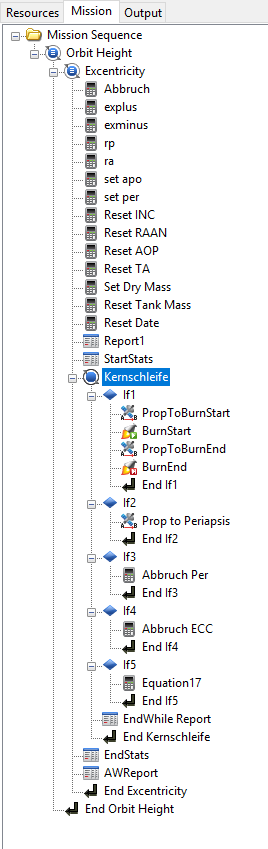
\includegraphics[width=0.35\textwidth]{graphics/GMAT/GMAT_Skript_ECC.PNG}
		\caption{Deorbitskript - Variation der Exzentrizität}
			\label{fig:GMAT_Skript_ECC}
\end{figure}



%-------------------------------------------------------------Ergebnisse
\newpage

\section{Ergebnisse}
Im Folgenden werden die Ergebnisse der zwei durchgeführten Simulationsarten präsentiert.
\begin{figure}[h]
\centering
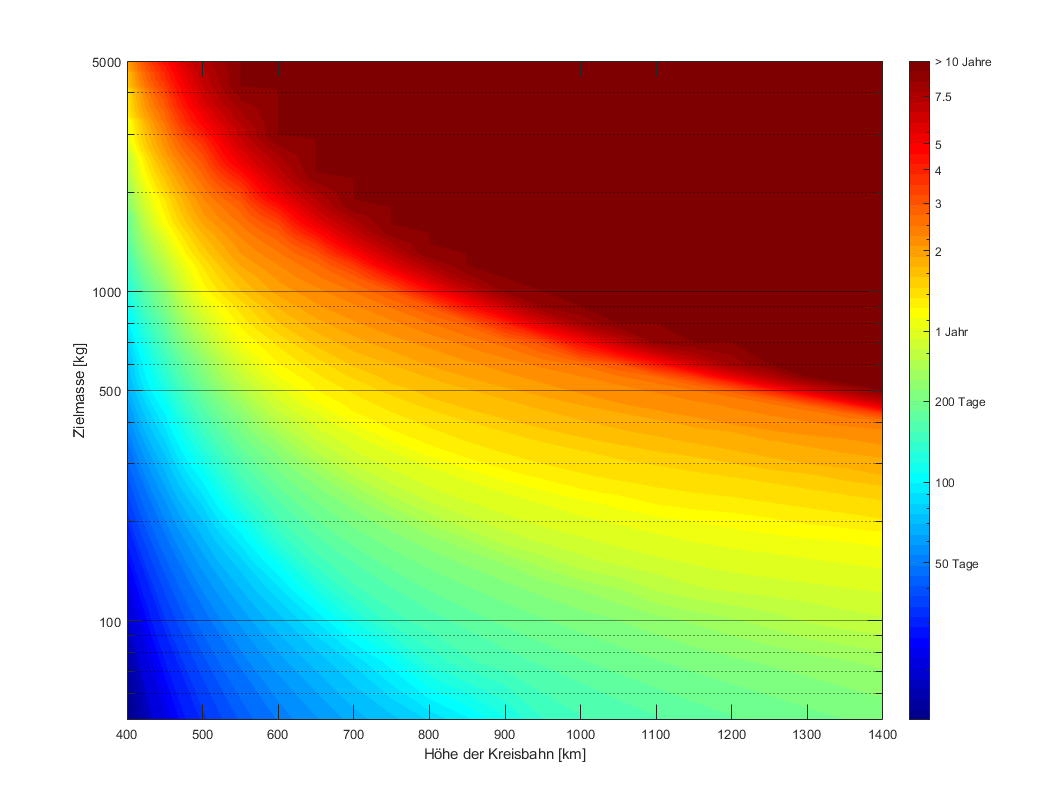
\includegraphics[width=1.00\textwidth]{./graphics/GMAT/GMAT_Mass_over_Height.png}
\caption{Simulationsergebnisse 50-5000kg, Kreisorbit}
\label{fig:GMAT_Mass_over_Height}
\end{figure}

\subsection{Beschreibung Mission 1}
In Abb. \ref{fig:GMAT_Mass_over_Height} sind die zugehörigen Deorbitzeiten farblich in Abhängigkeit von Masse und Starthöhe abgetragen. Die Zeitskala ist logarithmisch von 0 bis 10 Jahre an der Seite aufgeführt.  
Es ist klar zu erkennen, dass je niedriger die Masse, desto größer ist die Reichweite der Zielmassen, die innerhalb von zehn Jahren aus der Erdumlaufbahn entfernt werden kann.


Eine detaillierte Ansicht der Massen von 50 bis 550kg bietet \abb{fig:GMAT_Mass_over_Height_550}, da diese mit einer viermal höheren Auflösung (25kg Schritte) simuliert worden ist. Hier wird es deutlicher, dass die Zielmasse bei 1400km maximal 500kg betragen darf, um das Limit von zehn Jahren nicht zu überschreiten.

\begin{figure}[h!]
	\centering
		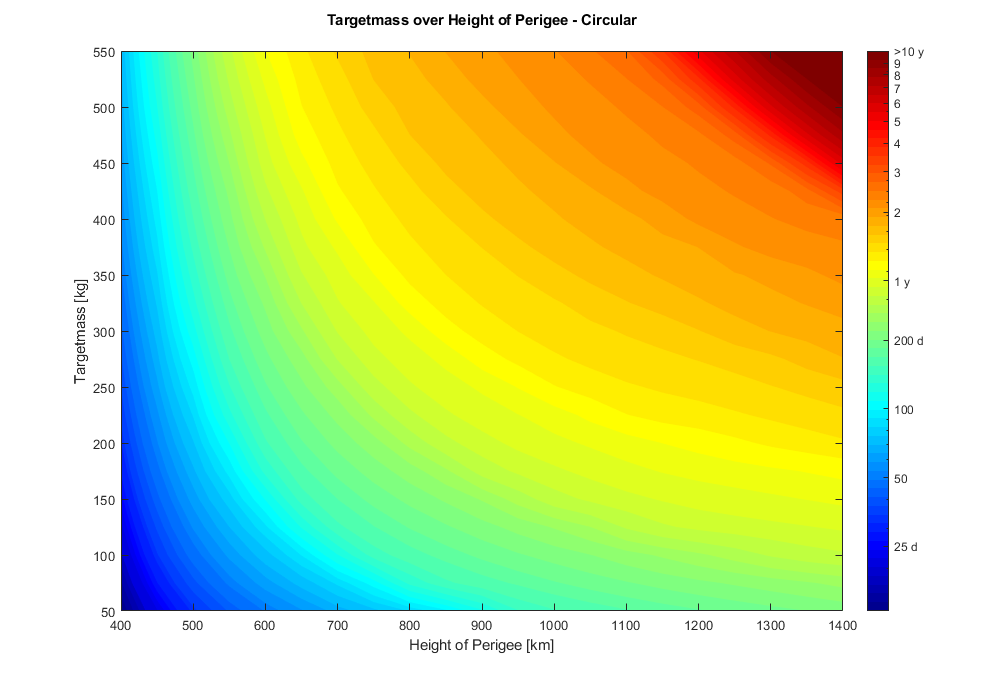
\includegraphics[width=1.00\textwidth]{./graphics/GMAT/GMAT_Mass_over_Height_550.png}
		\caption{Simulationsergebnisse 50-550kg, Kreisorbit}
	\label{fig:GMAT_Mass_over_Height_550}
\end{figure}


Durch die logarithmische Skala der Zeit ist klar erkennbar wie sehr die benötigte Zeit für die Mission ansteigt, nach dem der Treibstoff aufgebraucht worden ist. Dies geschieht im Bereich um drei Jahre. Je höher die Starthöhe, desto länger brennt das Triebwerk pro Umlauf, da die 58° Brennwinkel mehr Zeit benötigen um durchlaufen zu werden. 

\subsection{Ergebnis Mission 1}
Die gewählte Konfigurationen kann Satelliten mit einem Gewicht von 375kg(Starlink) innerhalb von 2 Jahren aus einer Erdumlaufbahn von 1400km aktiv zum Wiedereintrittverhelfen. Für niedrigere Höhen ist dieser Vorgang in weniger Zeit abgeschlossen. 


Bei großen Höhen ist die maximale Masse limitiert, jedoch ist der Aerodynamische Widerstand in geringen Höhen so stark, dass Trümmerteile bis zu zwei Tonnen innerhalb eines Jahres aus ihrer Umlaufbahn entfernt werden können. 

\subsection{Beschreibung Mission 2}

Die Abbildungen \ref{fig:GMAT_ecc_a}, \ref{fig:GMAT_ecc_b} und \ref{fig:GMAT_ecc_c} repräsentieren die Ergebnisse für die ausgewählten Massen 50, 375 und 550 kg. Die benötigte Missionszeit wird hier in Abhängigkeit von Exzentrizität und Starthöhe des Perigäums dargestellt. Die Zeitskala ist wieder logarithmisch von 0 bis zehn Jahre an der Seite aufgeführt.


\begin{figure}[h!]
	\centering
		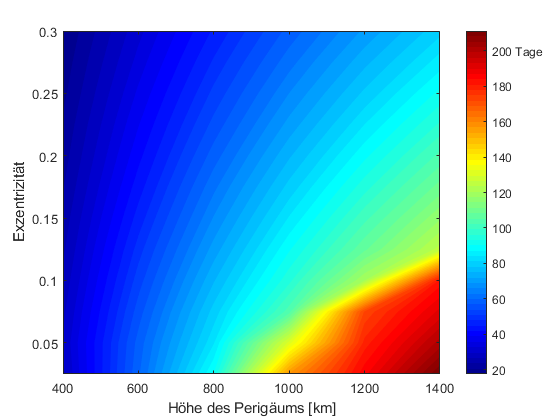
\includegraphics[width=1.00\textwidth]{./graphics/GMAT/ecc_perigee_50kg.png}
		\caption{Simulationsergebnisse Variation der Exzentrizität 50 kg}
	\label{fig:GMAT_ecc_a}
\end{figure}

\begin{figure}[h!]
	\centering
		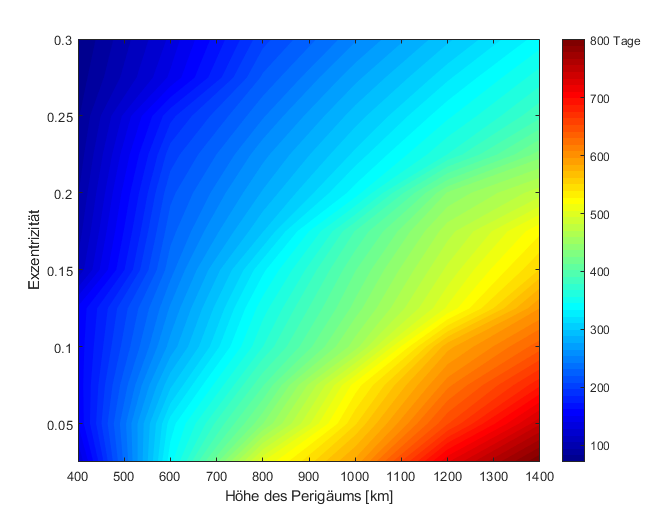
\includegraphics[width=1.00\textwidth]{./graphics/GMAT/ecc_perigee_375kg.png}
		\caption{Simulationsergebnisse Variation der Exzentrizität 375 kg}
	\label{fig:GMAT_ecc_b}
\end{figure}

\begin{figure}[h!]
	\centering
		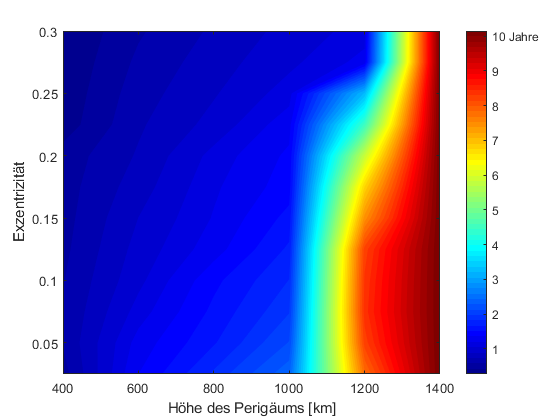
\includegraphics[width=1.00\textwidth]{./graphics/GMAT/ecc_perigee_550kg.png}
		\caption{Simulationsergebnisse Variation der Exzentrizität 550 kg}
	\label{fig:GMAT_ecc_c}
\end{figure}


Auffallend ist die Tatsache, dass eine höhere Exzentrizität eine geringere Missionszeit zur Folge hat. Der Grund hier für ist unter Anderem, dass bei hohen Exzentrizitäten der CubeSat länger innerhalb der 58° um das Apogäum ist und das Triebwerk somit länger brennen lassen kann. Im Fall von 550 kg zeigt \abb{fig:GMAT_ecc_550}, dass obwohl es über alle Höhenstufen zu einer verkürzung der Mission kommt, dies für 1400 km trotzdem über 10 Jahre dauert.



%For every considered satellite design (=mainly thruster configuration, 3-4 different designs), generate following data: \\
%
%Deorbit time and spent fuel mass for all:
%\begin{itemize}
	%\item Masses from 50-500 kg\\
	%\item Altitudes from 1400-400? km  (ggf. semi-major axis) \\
	%\item Eccentricities from ~0 to highest recorded eccentricity of debris in <1400 km orbit
%\end{itemize}
%
%Note: Output EVERY relevant simulation parameter (initial orbit and S/C data, burn start/stop angles, start epoch etc.)  at the beginning of every simulation run [discuss with Max]
	%
			%\subsection{Reachability Enveloppe}
%RESULTING DIAGRAMS: \\
%
%\begin{enumerate}
		%\item Visualize the absolute performance of the main design (Max), e = 0 \\
				%\begin{itemize}
						%\item Axes: y = mass, x = SMA \\
						%\item Graph: Use color gradients to display deorbit times (same time = same color)
				%\end{itemize}
				%\item  Visualize the influence of eccentricity on deorbit times using the main design \\
				%\begin{itemize}
						%\item Axes: y = mass, x = SMA \\
						%\item Select a fixed deorbit time (e.g. 2 years) \\
						%\item Graph: Use color gradients to display eccentricities (same ecc = same color)
				%\end{itemize}
				%\item Visually compare the performances of the different designs (Max \& 2-3 group designs), e = 0 
				%\begin{itemize}
						%\item Axes: y = mass, x = SMA \\
						%\item Select 1-2 fixed deorbit times (e.g. 2 years \& 5 years) \\
						%\item Graph: Draw lines of same deorbit time (selected above) for each of the different designs
				%\end{itemize}				
%\end{enumerate}
%Optional for group after 3. (decide if worth it)\\
%4. Repeat 1. with all other chosen designs\\
%
%NOTES: \\
%
%For 1. \& 4.:\\
%(Deorbit time limited to 10 years (15? 20?)) \\
%-> <2 years of deorbiting takes 3-4 mins to simulate, amount of data is immense => limit maximum deorbit time? \\
%-> At which deorbiting time does a feasible solution become unattractive? If 200 kg in 1000 km orbit is \\
   %deorbitable in 20 years, is it worth it? Better use chemical deorbiting = different mission in this case? \\
%---> Agree on a meaningful limit on deorbit time \\
%
%For all graphs/simulations: \\
%Fuel mass limited by design -> if 27U standard is to be kept no matter which thruster configuration is \\
%chosen, then smaller/more lightweight thrusters would result in more available space for fuel \\
%---> Agree on a set percentage of margin for all designs (e.g. 50\%) and determine maximum fuel from there? \\
%
%-> For Max's design, fuel mass limited to 10 kg (thinking about increasing to 15 kg)\\
			%\subsection{Missionsauslegung}
					%\textbf{Mögliche CubeSat Konfigurationen}\\
			%\subsection{Missionssimulation}
					%\textbf{Impuls-basierter Schub}\\
					%\textbf{Begrenzter Schub}\\
					%\textbf{Mission mit Randbedingungen}\\
			%\subsection{Konfigurationsvergleich}
					%\textbf{..}\\
					%\textbf{..}\\
					%\textbf{..}\\